%%%%%%%%%%%%%%%%%%%% author.tex %%%%%%%%%%%%%%%%%%%%%%%%%%%%%%%%%%%
%
% sample root file for your "contribution" to a contributed volume
%
% Use this file as a template for your own input.
%
%%%%%%%%%%%%%%%% Springer %%%%%%%%%%%%%%%%%%%%%%%%%%%%%%%%%%


% RECOMMENDED %%%%%%%%%%%%%%%%%%%%%%%%%%%%%%%%%%%%%%%%%%%%%%%%%%%
\documentclass[graybox,natbib]{svmult}

%%%% workaround for a pandoc issue
\def\tightlist{}



% choose options for [] as required from the list
% in the Reference Guide
%% The amssymb package provides various useful mathematical symbols
\usepackage{amssymb,amsmath}

\usepackage{mathptmx}       % selects Times Roman as basic font
\usepackage{helvet}         % selects Helvetica as sans-serif font
\usepackage{courier}        % selects Courier as typewriter font
\usepackage{type1cm}        % activate if the above 3 fonts are
                            % not available on your system
%
\usepackage{makeidx}         % allows index generation
\usepackage{graphicx}        % standard LaTeX graphics tool
                             % when including figure files
\usepackage{multicol}        % used for the two-column index
\usepackage[bottom]{footmisc}% places footnotes at page bottom

\usepackage{lipsum}
\usepackage{url}
\usepackage{gitinfo}
\usepackage[section,ruled]{algorithm}
\usepackage{algorithmic}
\usepackage{boxedminipage}
\usepackage[xetex,bookmarks=true,linkcolor=blue,hyperfootnotes=false,breaklinks=true,citecolor=blue,colorlinks=true]{hyperref}
\usepackage{sistyle}
\usepackage{xspace}
\SIthousandsep{,}

% see the list of further useful packages
% in the Reference Guide

\makeindex             % used for the subject index
                       % please use the style svind.ist with
                       % your makeindex program

%%%%%%%%%%%%%%%%%%%%%%%%%%%%%%%%%%%%%%%%%%%%%%%%%%%%%%%%%%%%%%%%%%%%%%%%%%%%%%%%%%%%%%%%%

\begin{document}
\motto{Manuscript version: \gitCommitterDate: \gitAbbrevHash\xspace -- draft for Electronic Symposium, ``Evolutionary Archaeologies: New Approaches, Methods, And Empirical
Sufficiency'' at the Society for American Archaeology conference, April 2016}

\title*{Measuring Cultural Relatedness Using Multiple Seriation Ordering Algorithms}
\titlerunning{Cultural Relatedness Through Multiple Seriation Algorithms}
% Use \titlerunning{Short Title} for an abbreviated version of
% your contribution title if the original one is too long
\author{Mark E. Madsen and Carl P. Lipo}
\institute{Mark E. Madsen \at Dept. of Anthropology, University of Washington, Box 353100, Seattle, WA 98195 \email{mark@madsenlab.org} \and Carl P. Lipo \at Environmental Studies Program and Dept. of Anthropology, Binghamton University, 4400 Vestal Parkway East
Binghamton, NY 13902-6000 \email{clipo@binghamton.edu}}

%
% Use the package "url.sty" to avoid
% problems with special characters
% used in your e-mail or web address
%
\maketitle



\abstract*{Seriation is a long-standing archaeological method for relative dating that has proven effective in probing regional-scale patterns of inheritance, social networks, and cultural contact in their full spatiotemporal context. The orderings produced by seriation are produced by the continuity of class distributions and unimodality of class frequencies, properties that are related to social learning and transmission models studied by evolutionary archaeologists. Linking seriation to social learning and transmission enables one to consider ordering principles beyond the classic unimodal curve. Unimodality is a highly visible property that can be used to probe and measure the relationships between assemblages, and it was especially useful when seriation was accomplished with simple algorithms and manual effort. With modern algorithms and computing power, multiple ordering principles can be employed to better understand the spatiotemporal relations between assemblages. Ultimately, the expansion of seriation to additional ordering algorithms allows us an ability to more thoroughly explore underlying models of cultural contact, social networks, and modes of social learning. In this paper, we review our progress to date in extending seriation to multiple ordering algorithms, with examples from Eastern North America and Oceania.}

\abstract{Seriation is a long-standing archaeological method for relative dating that has proven effective in probing regional-scale patterns of inheritance, social networks, and cultural contact in their full spatiotemporal context. The orderings produced by seriation are produced by the continuity of class distributions and unimodality of class frequencies, properties that are related to social learning and transmission models studied by evolutionary archaeologists. Linking seriation to social learning and transmission enables one to consider ordering principles beyond the classic unimodal curve. Unimodality is a highly visible property that can be used to probe and measure the relationships between assemblages, and it was especially useful when seriation was accomplished with simple algorithms and manual effort. With modern algorithms and computing power, multiple ordering principles can be employed to better understand the spatiotemporal relations between assemblages. Ultimately, the expansion of seriation to additional ordering algorithms allows us an ability to more thoroughly explore underlying models of cultural contact, social networks, and modes of social learning. In this paper, we review our progress to date in extending seriation to multiple ordering algorithms, with examples from Eastern North America and Oceania.}



\section{Introduction}\label{introduction}

Seriation is a set of methods which uses patterns in the occurrence or
abundance of historical classes to construct an ordering among otherwise
unordered assemblages or objects \citep{Dunnell:1970aa}. Traditionally,
the orders constructed by seriation were intended to be chronological,
since seriation was intended for use as a relative dating method by its
early 20th century developers
\citep{o2000applying, o1998james, Lyman:2006aa, OBrien1999b, lyman1997rise}.
But seriation techniques also create orderings which incorporate the
effects of spatial variation in addition to temporal change, as James
Ford pointed out \citep{Ford:1938aa, Phillips1951, Ford:1935aa}.

Despite the success of seriation in understanding the large-scale
structure of the archaeological record in the New World
\citep{Beals1945, Bluhm1951, Evans1955, Ford1949, Kidder1917, Mayer-Oakes1955, Meggers1957, Phillips1951, Rouse1939, Smith1950},
the method has largely been ignored since the advent of radiocarbon
dating given its primary association as a relative dating method. But
seriation is only a dating method in the sense that chronology is one
possible inference from mapping the spatiotemporal pattern of change in
cultural variants. Other inferences are possible, and in particular,
there is a growing understanding that seriation is one of several
methods for inferring historical and heritable continuity and thus
documenting the evolutionary history of past populations
\citep[e.g.,][Ch. 3]{OBrien1999b}.

Similarity between classes of artifacts constitutes heritable continuity
when it arises from information being passed between populations over
time; that is, from cultural transmission processes. Although the fact
that seriation, in some sense, measures cultural transmission has been
implicit since the earliest discussions of the method, the connection
remained a common sense generalization until the mid 1990's. Fraser
Neiman, in his dissertation and later his seminal 1995 article, noted
that the unimodal patterns that form the core of the traditional
frequency seriation technique are regularly seen in the trajectories
seen when simulating unbiased transmission \citep{Neiman1995}. In order
to make this connection both rigorous and useful in empirical work, we
began a research program aimed at exploring the connection between
cultural transmission models and seriation methods
\citep{Lipo1997Population}, which has resulted in numerous publications,
new seriation software algorithms, and many conference papers
\citep{huntmadsenlipo1995a, lipomadsenhunt1995b, Lipo2008, Lipo2001, Lipo2001a, Lipo2005, lipomadsen1997, lipomadsendunnell2015, Madsen2014, madsenlipo2015b, Madsen2008, o2015design}.

The core of the all seriation techniques are a set of ``ordering
principles'' which describe how the data points making up each
assemblage or object are rearranged in order to achieve a valid
seriation solution. Traditionally, there are two
\citep{Dunnell:1970aa, Rouse1967, Whitlam:1981vs}. The ``occurrence
principle'' states that a valid ordering leaves no temporal gaps in the
distribution of the historical classes used, and thus that temporal
orders are continuous
\citep{dempsey1963statistical, rowe1959archaeological}. The ``frequency
principle'' states that in a valid ordering, the frequencies making up
the continuous distribution of each historical type will be unimodal,
possessing a single peak of ``popularity'' \citep{Nelson1916}.

Both principles work, as demonstrated by the robustness and continued
utility of the basic chronological frameworks erected by culture
historians in the first half of the 20th century using seriation along
with stratigraphy and marker types \citep{lyman1997rise}. The frequency
principle remains, however, an empirical generalization which is only
suggested by the behavior of cultural transmission models, rather than
being a necessary consequence. This suggests to us that seriation as a
method requires further methodological development, especially if it is
to be one of our major tools in tracing historical and heritable
continuity in the archaeological record.\footnote{Cladistics and
  phylogenetic methods, especially those which take into account
  temporal differences in the samples being studied (stratocladistics)
  and which are capable of yielding phylogenetic networks in addition to
  trees, are the other major tools by which we can measure heritable and
  historical continuity.}

INTRODUCTION INCOMPLETE UNTIL LATER SECTIONS DRAFTED

\section{Seriation and the Frequency
Principle}\label{seriation-and-the-frequency-principle}

Seriation, in the Americanist sense, was initially developed by Alfred
Kroeber \citep{Kroeber1916} in the Southwest, on the basis of changes in
ceramic decorations from Zuni Pueblo. The primitive seriation proposed
by Kroeber was quickly amended by Leslie Spier, Alfred V. Kidder and
Nels C. Nelson all of whom were conducting stratigraphic excavations in
the American Southwest \citep{Kidder1917, Nelson1916, Spier1917}. This
group of researchers all noticed that when ceramics were described in a
particular way -- called ``stylistic'' by Kidder
\citeyearpar{Kidder1917} -- the temporal distribution of the types took
the form of ``normal curves.'' Using such types, it was apparent that a
series of assemblages collected from the surface or otherwise undated
could be arranged in chronological order by rearranging them so that all
type distributions approximated ``normal curves'' simultaneously. The
orders constructed in this way could also be tested by finding
stratified deposits and were found to be correct.

As powerful as seriation proved to be, these early formulations were
entirely intuitive and based on the generalization that greater temporal
differences between assemblages caused larger differences between
frequencies of decorated types, and that properly constructed historical
types displayed a clear pattern of change \citep[p.~220]{Phillips1951}:

\begin{quote}
If our pottery types are successful measuring units for a continuous
stream of changing cultural ideas, it follows that when the relative
popularity of these types is graphed through time, a more or less long,
single-peak curve will usually result. Put in another way, a type will
first appear in very small percentages, will gradually increase to its
maximum popularity, and then, as it is replaced by its succeeding type,
will gradually decrease and disappear.
\end{quote}

This compactly describes the ``popularity principle,'' originally
articulated by Nelson \citeyearpar{Nelson1916} and Wissler
\citeyearpar{wissler1916application}. A key word in the above is
``usually,'' since not all types display the unimodal distribution
described, even when the attributes chosen are explicitly stylistic and
decorative. Types suitable for frequency seriation were a subset of
stylistic variation, comprising those which displayed spatial and
temporal contiguity, a long enough duration that the types overlapped in
their representation among sites and assemblages, and those whose
distribution through time displayed the characteristic unimodal form
which allowed the analyst to arrange them by eye. The process of
constructing and testing such types became known, after Krieger
\citeyearpar{Krieger1944}, as applying the ``test of historical
significance.''

\subsection{Unimodality and Cultural Transmission
Processes}\label{unimodality-and-cultural-transmission-processes}

In most cases (such as the above quote from Phillips, Ford, and
Griffin), the popularity principle is simply assumed to hold in
culture-historical applications. It is clear that culture historians
assumed that what generates heritable continuity, and thus allows the
tracing of chronological relations, is cultural transmission. As Lyman
\citeyearpar{Lyman2008} documents in careful detail, early 20th century
anthropology and archaeology understood and discussed a variety of
transmission processes informally, as generating the patterns they
studied, even if they used different terms and did not form quantitative
models for it. Rouse \citeyearpar{Rouse1939}, for example, explicitly
discussed the diffusion of cultural traits, in terms that we now
recognize as a spatiotemporal model of transmission. Kroeber, the father
of frequency seriation, clearly understood the connection between his
previous work and trait diffusion \citep{kroeber1937diffusion}. There
are many more examples \citep{Lyman2008}.

It was not until archaeologists began working with stochastic models of
cultural transmission, however, that we could easily visualize the sheer
variety of patterns that cultural transmission processes can, and do,
generate. Archaeologists had long had quantitative models of diffusion
\citep[e.g.,][]{ammerman1971measuring}, but Dunnell's
\citeyearpar{Dunnell1978} exposition of style as neutral variation led
to adoption of stochastic models of drift from population genetics as
the main tool for exploring cultural transmission dynamics. Many
previous models of diffusion tended to be deterministic, especially
those stemming from the interdisciplinary literature on the diffusion of
innovations \citep[e.g.,][]{Rogers2003}. Neiman \citeyearpar{Neiman1995}
simulated drift in cultural variants as an unbiased transmission
process, as shown in Figure \ref{img:neiman-fig2}. Immediately apparent
is the fact that some variants do display unimodal patterns, but most
variants are multimodal or display violations of unimodality at small
scales even if the macroscopic shape seems to conform to the popularity
principle.

\begin{figure}[ht]
\centering
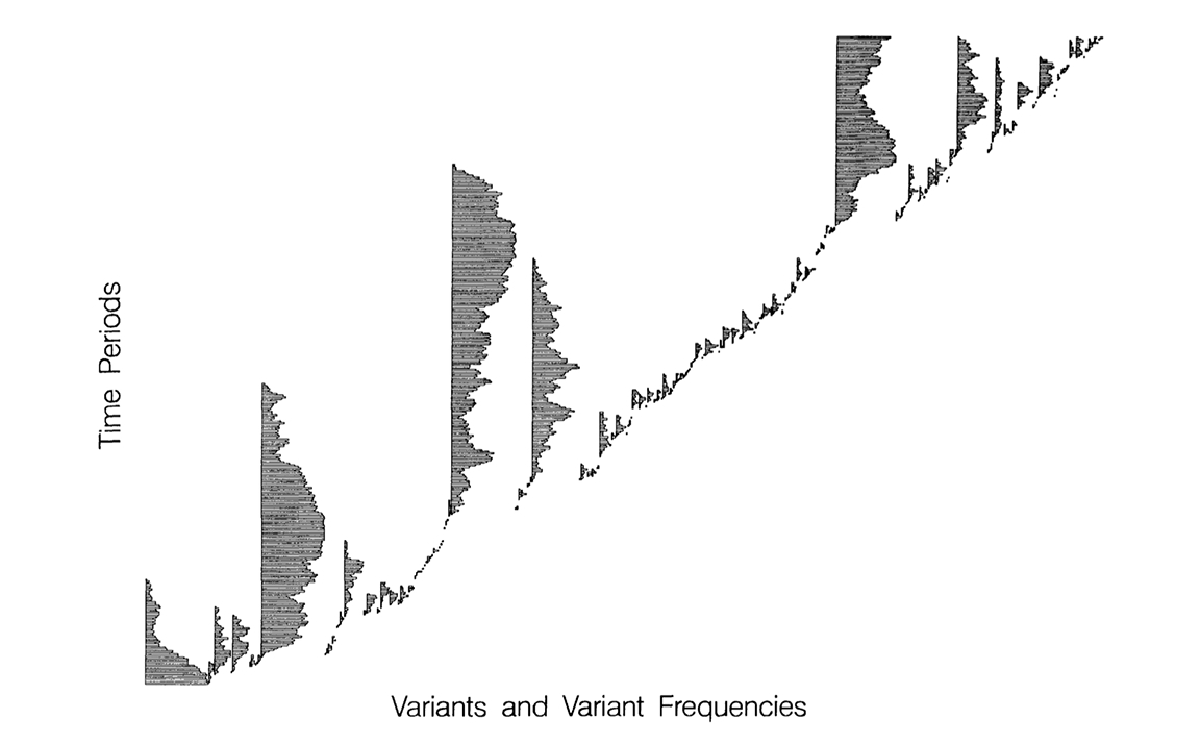
\includegraphics[scale=0.6]{neiman-1995-figure2a.pdf}
\caption{Neiman's simulation of drift in cultural variant frequencies under unbiased cultural transmission (reproduction of Figure 2a from Neiman 1995.)}
\label{img:neiman-fig2}
\end{figure}

The lesson of Figure \ref{img:neiman-fig2} is that there is nothing
necessary about unimodality given cultural transmission, but that it can
occur. But culture historical types used in seriation were
\textbf{constructed} to yield unimodal distributions, and a key element
in such construction is ensuring that types are composed of multiple
dimensions of variation which co-occur on artifacts identified to that
type. We can imagine selecting the traits shown in Figure
\ref{img:neiman-fig2} and intersecting combinations of them to form
multidimensional classes. In doing so, it is likely that unique
combinations of those variants would not recur and might show unimodal
distributions more often. It is also likely that time averaging
(ubiquitous in the archaeological record) will smooth out some of the
minor variation in variant frequencies, as will the vagaries of sampling
archaeological deposits.

Taken together, these factors seem to explain why the intuitive
construction of historical types, from the continuous flow of the
products of cultural transmission processes, worked to produce
chronology through application of the common-sense popularity principle,
and why not all artifact classes constructed from otherwise
``stylistic'' dimensions of variation, are suitable for frequency
seriation using unimodality as the ordering criterion.

\subsection{Continuity: An Alternative to
Unimodality}\label{continuity-an-alternative-to-unimodality}

There are several reasons why we should explore alternatives to
unimodality as an ordering algorithm for frequency seriation. First,
from a performance perspective, searching for unimodal orders is
computationally expensive, even for relatively small data sets
\citep{Madsen2014}. Even with the iterative, agglomerative method that
we introduced recently \citep{lipomadsendunnell2015}, the computation
time can diverge for data sets as small as 30. This is a large number of
assemblages by most archaeological standards, but with good techniques
and ordering principles seriation may scale to much larger problems, and
even be applicable to the flood of data seen in modern day life.

Second, and more importantly from a theoretical perspective, it is
important to be able to trace heritable continuity even if does not
display a particular type of temporal frequency distribution. Using
traditional type construction methods and the test of historical
significance, culture historians were able to find \textbf{enough}
conforming types and classes to construct regional chronologies. But
there is a strong relationship between the number of classes in a
seriation, and our ability to map differences across space and time. The
use of seriation as a method for tracing evolutionary relationships is a
more demanding task than establishing rough chronology in a region.
Thus, it is worth searching for additional ordering principles that may
be useful for seriating more classes of cultural variants.

A theoretically sound ordering principle for seriation should be
derivable from characteristics of the underlying cultural transmission
processes that we believe drive the spatiotemporal variation seriation
measures. Formal models of cultural transmission, such as those
formulated by Boyd and Richerson, Cavalli-Sforza and Feldman, and
borrowed from population genetics
\citep{Boyd1985, Cavalli-Sforza1981, Neiman1995} are stochastic
autoregressive processes, in the sense that the probability distribution
of outcomes at a given time are dependent upon the outcomes from the
immediate past. Mathematically, we usually formulate cultural
transmission models as Markov processes, usually of first order (i.e.,
without dependencies on states previous to the immediate past state).
Such models are certainly capable of making large changes in state over
short time intervals, but large jumps are rare compared to small changes
in state, especially in large populations.This is the reason why we (and
culture historians) often have an expectation that cultural transmission
has a ``gradual'' character to it.

The probabilistic gradualism of change over small time periods in our
cultural transmission processes suggests a ``continuity'' principle,
strongly related to notions of continuous functions in mathematics:
samples which originate close together in time, space, or both will be
close in type frequency and the presence/absence of types, especially
compared to samples which are further apart. This continuity principle
immediately leads to considering ordering algorithms based upon
minimizing a suitable distance metric, with assemblages represented by
points in a multidimensional space of type frequencies or counts.

\subsection{Statistical Seriation
Methods}\label{statistical-seriation-methods}

The earliest statistical techniques for seriation were also built upon
using interassemblage distance metrics. Brainerd and Robinson
\citep{Brainerd1951, Robinson1951} pioneered a method for seriation
based upon the similarity between assemblages, measured as a scaled
version of the Manhattan (or city-block) distance between assemblage
frequencies. When these scaled distances (which became known as
Brainerd-Robinson coefficients) are arranged in a matrix with the
largest values nearest the diagonal and the lowest values in the corners
and away from the diagonal, the order of assemblages by row or column
provides the seriation solution. In practice, most real data matrices
cannot be put in perfect Robinson form without violations.

What followed Brainerd and Robinson's pioneering work was a minor
industry in methods for matrix ordering, in the face of the practical
difficulties in coercing most data sets into a perfect linear ordering
\citep[e.g.,][]{dempsey1963statistical, Kendall1963, Matthews1963, Bordaz1970aa, Gardin1970, Kendall1970, Kendall1971}.
As access to computers by researchers in the social sciences increased,
computerized algorithms for examining permutations quickly proliferated
\citep{Ascher1963, craytor1968refinements, Kuzara1966}. Kendall
\citeyearpar{Kendall1969} and others attacked the ordering problem
through the use of multidimensional scaling, and later correspondence
analysis would be used with success in determining probabilistic
seriation orders, and just as importantly, quantifying the degree of
departure from the ideal seriation model \citep{Smith2005}. For a
detailed review of the many variants on this type of probabilistic
seriation solution, see \citep{Marquardt:1978aa}.

Not all of the similarity measures used in this literature are true
distance metrics, but many are, and there were calls to simplify the
problem by directly minimizing inter-assemblage distance, and thus the
total ``path length'' of a candidate seriation solution. Kadane
\citeyearpar{Kadane1971} describes this approach, and it was adopted
later by Shepardson \citeyearpar{shepardson2006} in his construction of
the ``Optipath'' seriation algorithm, which has distance minimization at
its core.

Where existing distance/similarity methods encounter a problem is the
assumption that a seriation solution must be a single linear order. In
an earlier paper, we describe a seriation algorithm (iterative
deterministic seriation solutions, or IDSS) that finds all of the
possible orders in a set of data that conform to an ordering principle,
and where those orders have overlap in assemblages, IDSS constructs a
graph with branches that recognizes that the best solutions may not be
linear \citep{lipomadsendunnell2015}. Departures from linear seriation
solutions have always been treated as ``stress'' or ``error,''
especially when statistical methods such as MDS or correspondence
analysis are employed. Practitioners usually recognize that such
departures arise from coercing data which naturally sit in a larger
number of dimensions -- because of spatial variation and other factors
-- into a one-dimensional order. In essence, methods which attempt to
coerce a complex spatiotemporal pattern into a linear ordering tend to
treat departures from linearity as noise, which is then ignored.

But the departure from linearity is not ``noise,'' in the statistical
sense. Especially if one accounts for sampling error in constructing
seriation orders (as we do in IDSS by using the bootstrap to construct
confidence intervals around the empirical frequencies), then departures
from a linear ordering are \textbf{signal}, not noise. Such solutions
reflect the fact that an assemblage at time \(T_1\), for example, may be
the closest match to two different assemblages at later times \(T_2\)
and \(T_3\) for example, given slightly different areas of overlap in
their type frequencies. This can occur because the seriation method is
inherently spatiotemporal, instead of simply measuring time (as culture
historians have always known), and it can also reflect the splitting of
populations into separate lineages (or their merger).

\subsection{\texorpdfstring{Exact Distance Minimization Ordering:
``Continuity''
Seriation}{Exact Distance Minimization Ordering: Continuity Seriation}}\label{exact-distance-minimization-ordering-continuity-seriation}

Instead of the ``approximate'' distance minimization algorithms employed
in multidimensional scaling and Shepardson's OptiPath seriation
software, we explore exact solutions using our IDSS software. For
simplicity in the configuration of the software, we summarize our
approach by calling it ``continuity'' seriation, to emphasize that we
want solutions that have the smoothest, most continous transition of
type frequencies when we consider pairs of assemblages. We achieve this
by locally minimizing the inter-assemblage distance within the solution
graph, which automatically yields the minimum total ``path length'' for
a seriation solution.

Our algorithm makes no use of the unimodality criterion, and produces
equivalent results in almost all cases, as we show in the next section.
The algorithm currently employs the Euclidean distance between
assemblage counts or frequencies, although it can use any distance
metric. Given a table of inter-assemblage distance metrics, we first
construct pairs of two-vertex graphs which represent the ``closest''
assemblage for each assemblage in the data set (mirrored pairs are
filtered out since they are isomorphic). The edge weight given to each
edge is the Euclidean distance between the assemblages represented by
vertices. For each of the minimal graphs in this initial set, we then
find the assemblage with the shortest distance to each of the two ends,
and continue iterating. Crucially, if there are equal-distance options,
both possible solutions are retained. The result of this iteration is a
collection of graphs which represent partial minimum-distance paths
through the set of assemblages. This collection of partial graphs are
then overlaid to form a single solution using a ``minmax'' approach as
described in our paper on the IDSS algorithm in general
\citep{lipomadsendunnell2015}.

The general approach is the same one we take to frequency seriation;
what differs here with ``continuity'' seriation is how we form the set
of candidate partial solutions. Instead of enforcing unimodality within
each partial solution, we minimize Euclidean inter-assemblage distance.
The resulting minmax graph is linear only if all of the candidate
partial solutions perfectly overlay themselves into a linear solution,
and otherwise will have a tree structure with branches. The possibility
of branching is what allows a seriation solution to express both spatial
and temporal structure simultaneously. The ability to inform on both
allows investigation of social network structure, and interaction and
social learning patterns in past populations, at scales more detailed
than entire cultural manifestations or phases. We believe that
seriation, augmented in this way, sits between the microevolutionary
level where we investigate evolution in single populations, and the
macroevolutionary level, best explored using the tools of phylogenetic
analysis and cladistic techniques.

\section{Comparing Frequency and Continuity
Seriation}\label{comparing-frequency-and-continuity-seriation}

In this section we compare the results of our IDSS frequency seriation
algorithm, described in a recent paper \citep{lipomadsendunnell2015},
and our exact distance-minimization or ``continuity'' algorithm. It is
difficult to compare the algorithms on a very large set of empirical
data sets, so we begin by examining a large sample of data sets
generated by sampling simulated cultural transmission, within a regional
metapopulation model of multiple communities. We described the overall
model, called ``SeriationCT,'' in a conference paper last year, but we
review the essentials here.\footnote{The SeriationCT software is open
  source, and is located at
  \href{https://github.com/mmadsen/seriationct}{Github}. Experiments
  using it to generate the data analyzed here, and more network models,
  are described and linked on
  \href{http://notebook.madsenlab.org}{Madsen's website and lab
  notebook}.}

Seriation of artifact assemblages is inherently a regional-scale
problem, whether for chronology or tracking interaction and social
learning processes. Thus, the fundamental abstraction for modeling is a
graph or network which (a) represents the intensity of contact,
migration, and interaction between communities of people at any given
point in time, (b) allows the set of communities to evolve, with some
communities going away and others originating over time, and (c)
representing how both the pattern and intensity of inter-community
contacts evolves over time. Social network or graph models, especially
weighted graphs, form an essential ingredient for this type of modeling,
but need to be extended to the temporal dimension.

Extending networks for modeling time-transgressive change employs
so-called ``temporal network models,'' which record the changing
structure a network or graph over a series of time points
\citep{Holme2012}. For our purposes, ``interval'' temporal networks are
the right abstraction. Such graphs represent interactions that occur and
persist over a measurable duration as edges that carry time indices.
Interval graphs can be modeled mathematically in a number of ways, but
in an algorithmic setting the most convenient is to define a sequence of
separate graphs, where each graph \(G_t\) in the sequence represents one
or more change events within the network between times \(t\) and
\(t + \delta t\) (where \(\delta t = t+1 - t\)). In a fully continuous
temporal representation, each graph in the sequence specifies a single
change event, and thus is equivalent to the way that a continuous-time
stochastic process represents events. In situations where our
observations are coarse grained due to time averaging or recovery
methods (or both), each graph in the sequence may represent a number of
change events which occur over the duration assigned to that graph in
the sequence.

Change events encompass anything that modifies the graph. Vertices may
be added or removed, and edges may be added or removed. In addition to
addition and removal, if the graphs in the sequence are weighted, slices
may record events where the strength of an edge changes, without other
topological changes to the graph. If other attributes are present on
vertices or edges (e.g., labeling edges for a type of interaction),
changes to those labelled attributes would also constitute a change
event and would be recorded by a graph in the sequence with changed
attribute values. An interval temporal network is thus defined as an
ordered set of graph ``slices,'' each slice associated with a time
index. The changes themselves can be found by ``subtracting'' two graph
slices and obtaining lists of vertex and edge changes.

Constructing a time-transgressive regional metapopulation from an
interval temporal network occurs by giving interpretations to vertices,
edges, and other attributes of the graph. In our research, vertices
represent communities of individuals, with population sizes which may
change or not over time. Edges represent the presence of interaction
between two communities, which could represent learning between
individuals, or migration of individuals bringing portions of a cultural
repertoire between communities. The weight given to an edge is typically
a relative measure of interaction betweeh communities, normalized by the
rest of the communities, since there is no good way in a simple
structure like this to model the absolute intensity of such interaction.
When communities come into existence, by members of an existing
community founding a new settlement, a vertex is added to the network
and it acquires connections to other communities (according to the class
of model we are constructing). Similarly, communities may go away over
time, and the vertex is then removed. Interaction patterns may change as
well, resulting in the addition or removal of edges over time, or change
in the edge weights.

For example, we can create a model whereby two clusters of communities
are tightly interconnected internally, and have some sparser
relationship between the clusters, and slowly lose that interconnection
to become separate, non communicating lineages, using a model similar to
that shown in Figure \ref{img:itn-example}.\\
The third and fourth columns in the figure describe the change events.
The third describes changes to the network structure in each time slice,
and the fourth describes the interpretation of those structural changes
in terms of a regional metapopulation model.

\begin{figure}[ht]
\centering
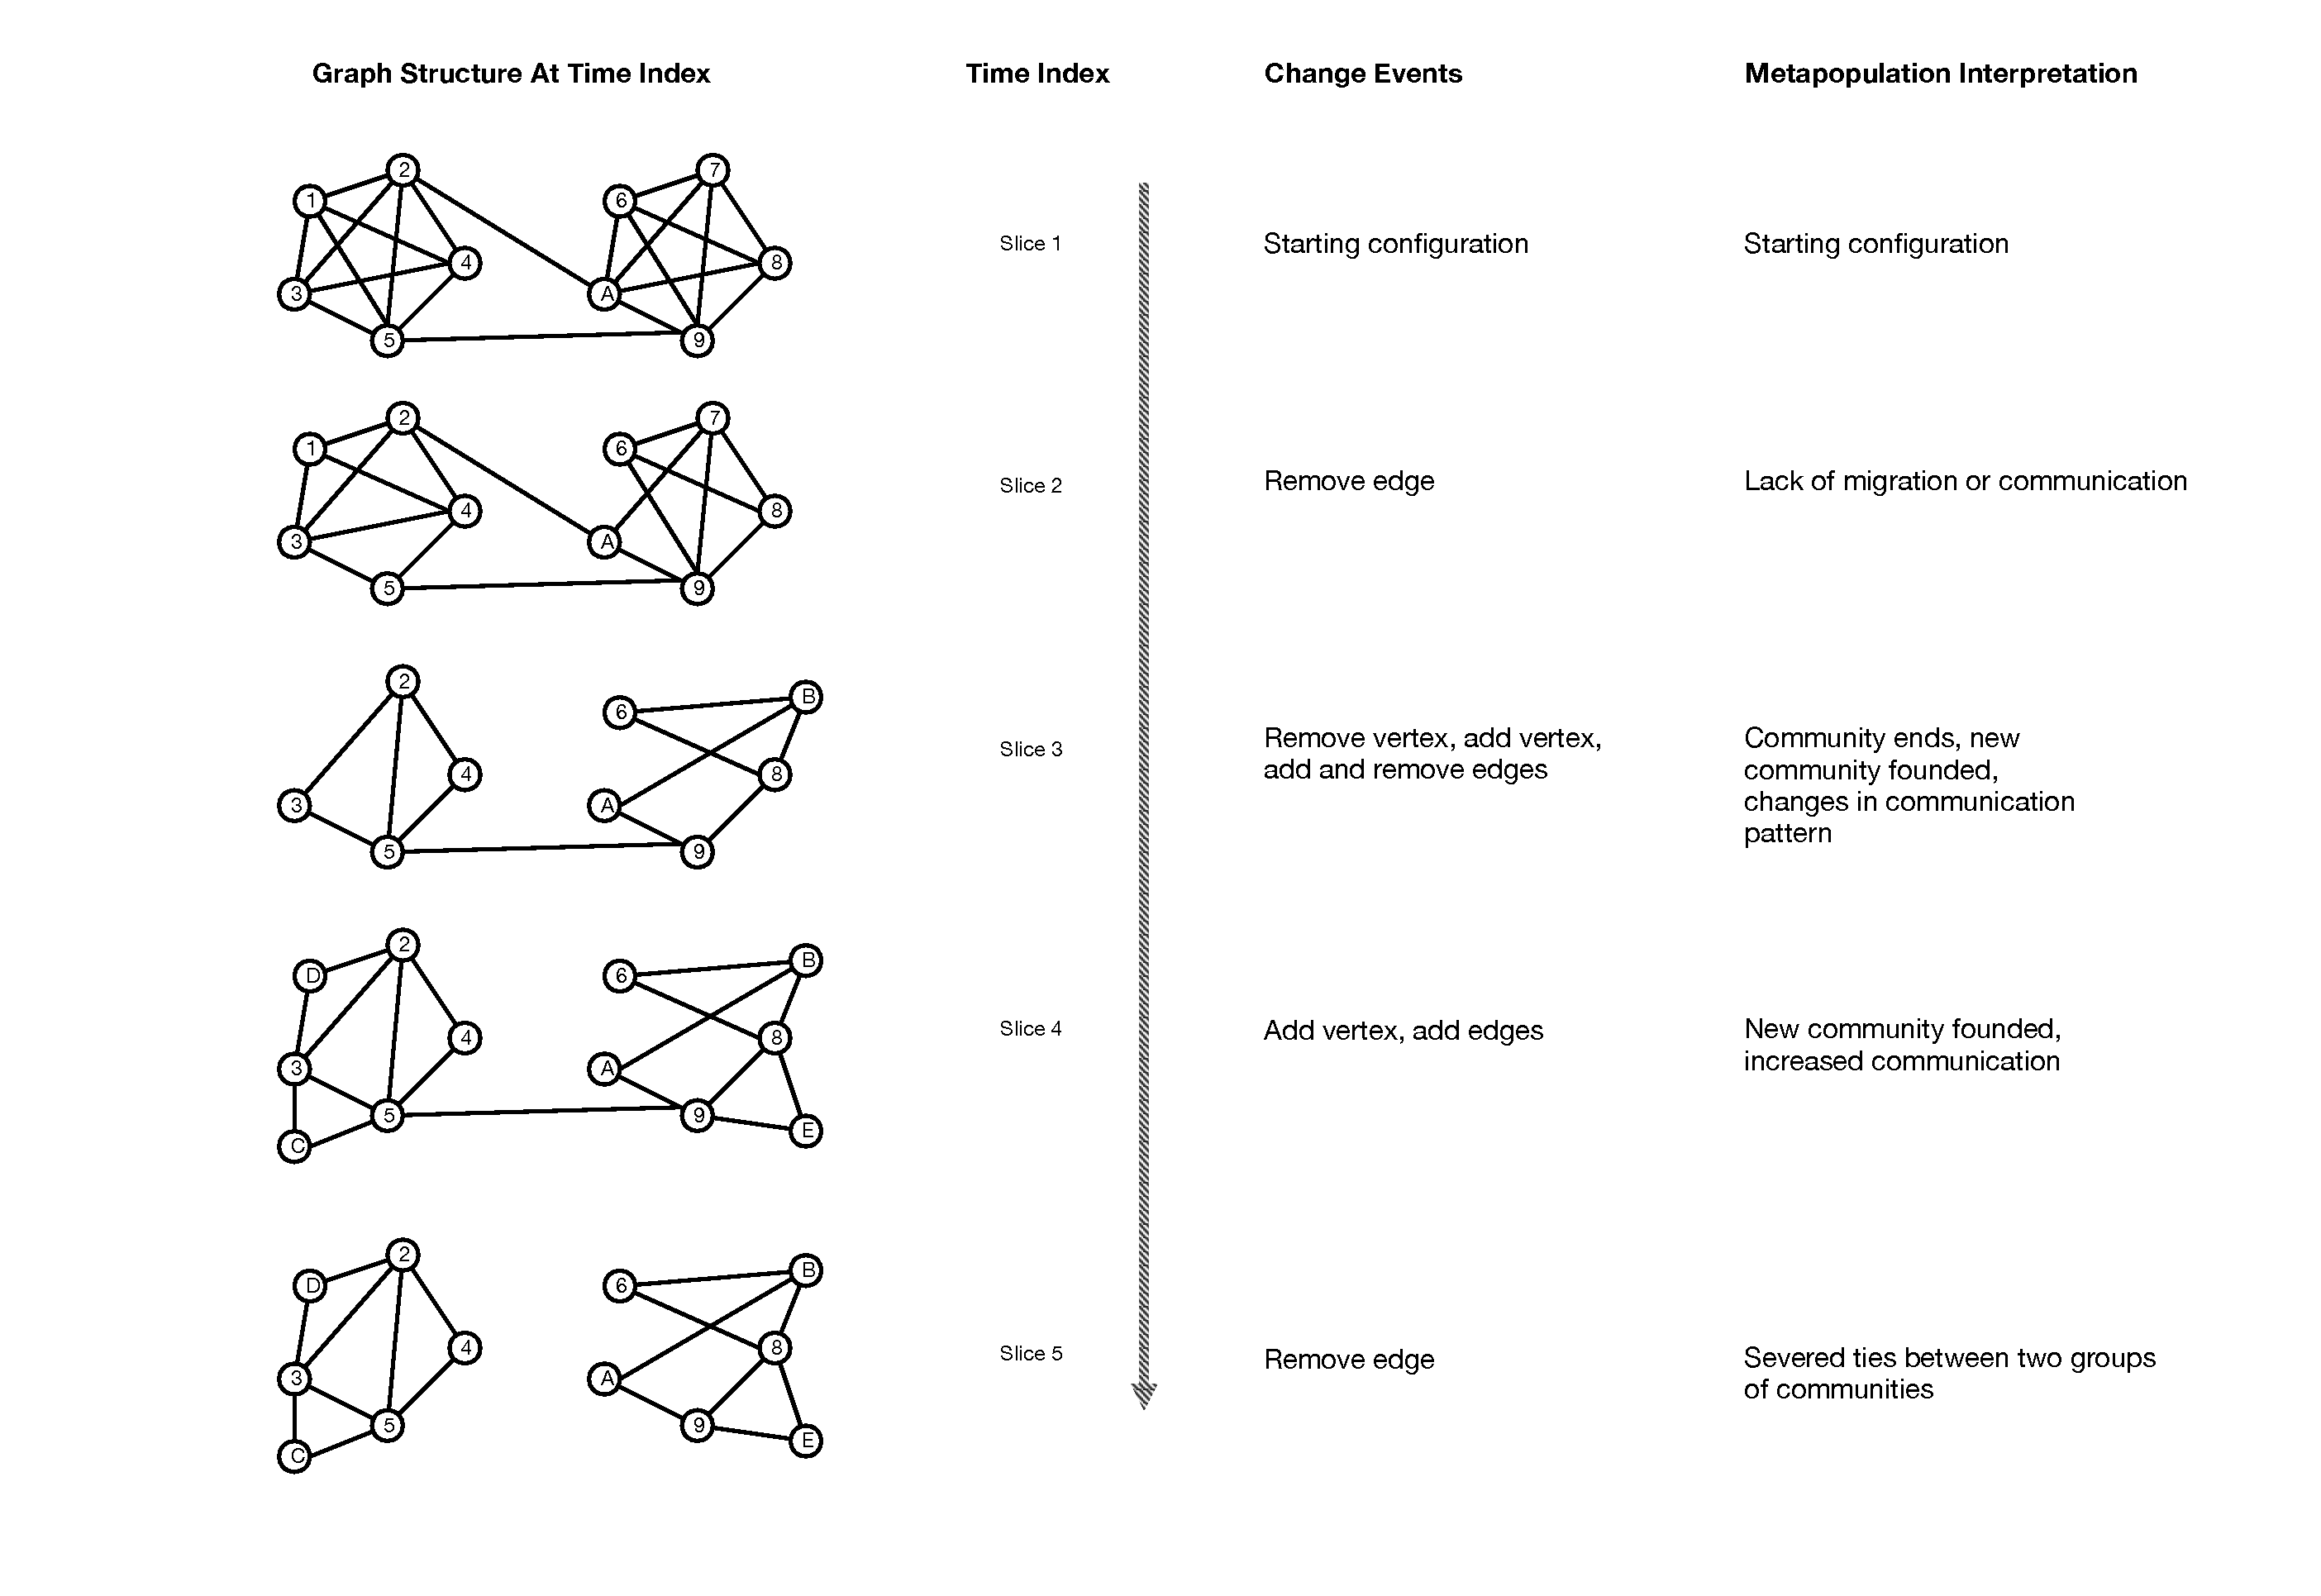
\includegraphics[scale=0.25]{interval-temporal-network-with-interpretation.pdf}
\caption{Example of an interval temporal network interpreted as a regional metapopulation model, with vertices representing communities, weighted edges representing intensity of interaction and migration, and changes in each representing their respective evolution over time.}
\label{img:itn-example}
\end{figure}

Interval temporal networks, interpreted as regional metapopulation
models, thus form a basic tool for modeling many classes of regional
histories and interaction patterns. For purposes of comparing frequency
and our continuity seriation algorithms, we focus on a regional model of
the type depicted in Figure \ref{img:itn-example}, but with a larger
number of communities than shown. In that model, four clusters of
communities start out at the beginning of the time period under
consideration being tightly interconnected within each cluster, and more
loosely connected among the four clusters. At any given time, each
cluster has 8 communities spread over a geographic area, so with four
clusters, there are 32 communities in the region under consideration. At
a late point in the time interval under consideration, the connections
between pairs of clusters is removed, creating two non-interacting sets
of community clusters, to model the origin of separate ``lineages'' of
cultural transmission in a region.\footnote{This model is available for
  inspection as a set of GML network files in experiment ``sc-2'' in the
  \href{https://github.com/mmadsen/experiment-seriation-classification}{experiment-seriation-classification}
  repository maintained by Madsen. That experiment focused on
  differentiating different classes of lineage-splitting or coalescence
  models through their seriation solutions, and here I focus only on the
  data resulting the ``late lineage splitting'' model.}

Given this model of interaction between communities, we then simulate
the standard unbiased cultural transmission model across this network.
The changes specified by the temporal network guide the addition of new
subpopulations or their demise in the model, and the edge weight pattern
defines migration of individuals between communities, and thus the
possibility of cultural variants flowing between communities. Simulation
of transmission occurs for 12,000 time steps, with the change events
occurring regularly over that interval, creating change in interaction
over time as social learning proceeds.

During the evolution of the model, we record the frequencies of
individual variants, and their co-occurrence to mimic archaeological
classes or types which are defined by multiple dimensions of variation.
Recording of frequencies occurs within each of the 32 communities
present at any given point in time, so we can measure spatial and
temporal variation in cultural variants. For purposes of the experiments
reported here, we sample innovation rates from a prior distribution
which allows any given simulation run to have a very low innovation
rate, through relatively high innovation rates.\footnote{The details of
  the prior parameter distributions are relatively unimportant for
  purposes of comparing seriation algorithms, but are found in the
  \href{https://github.com/mmadsen/experiment-seriation-classification}{experiment-seriation-classification}
  repository under experiment SC-2 in the file
  ``seriationct-priors.json''.}

\begin{figure}[ht]
\centering
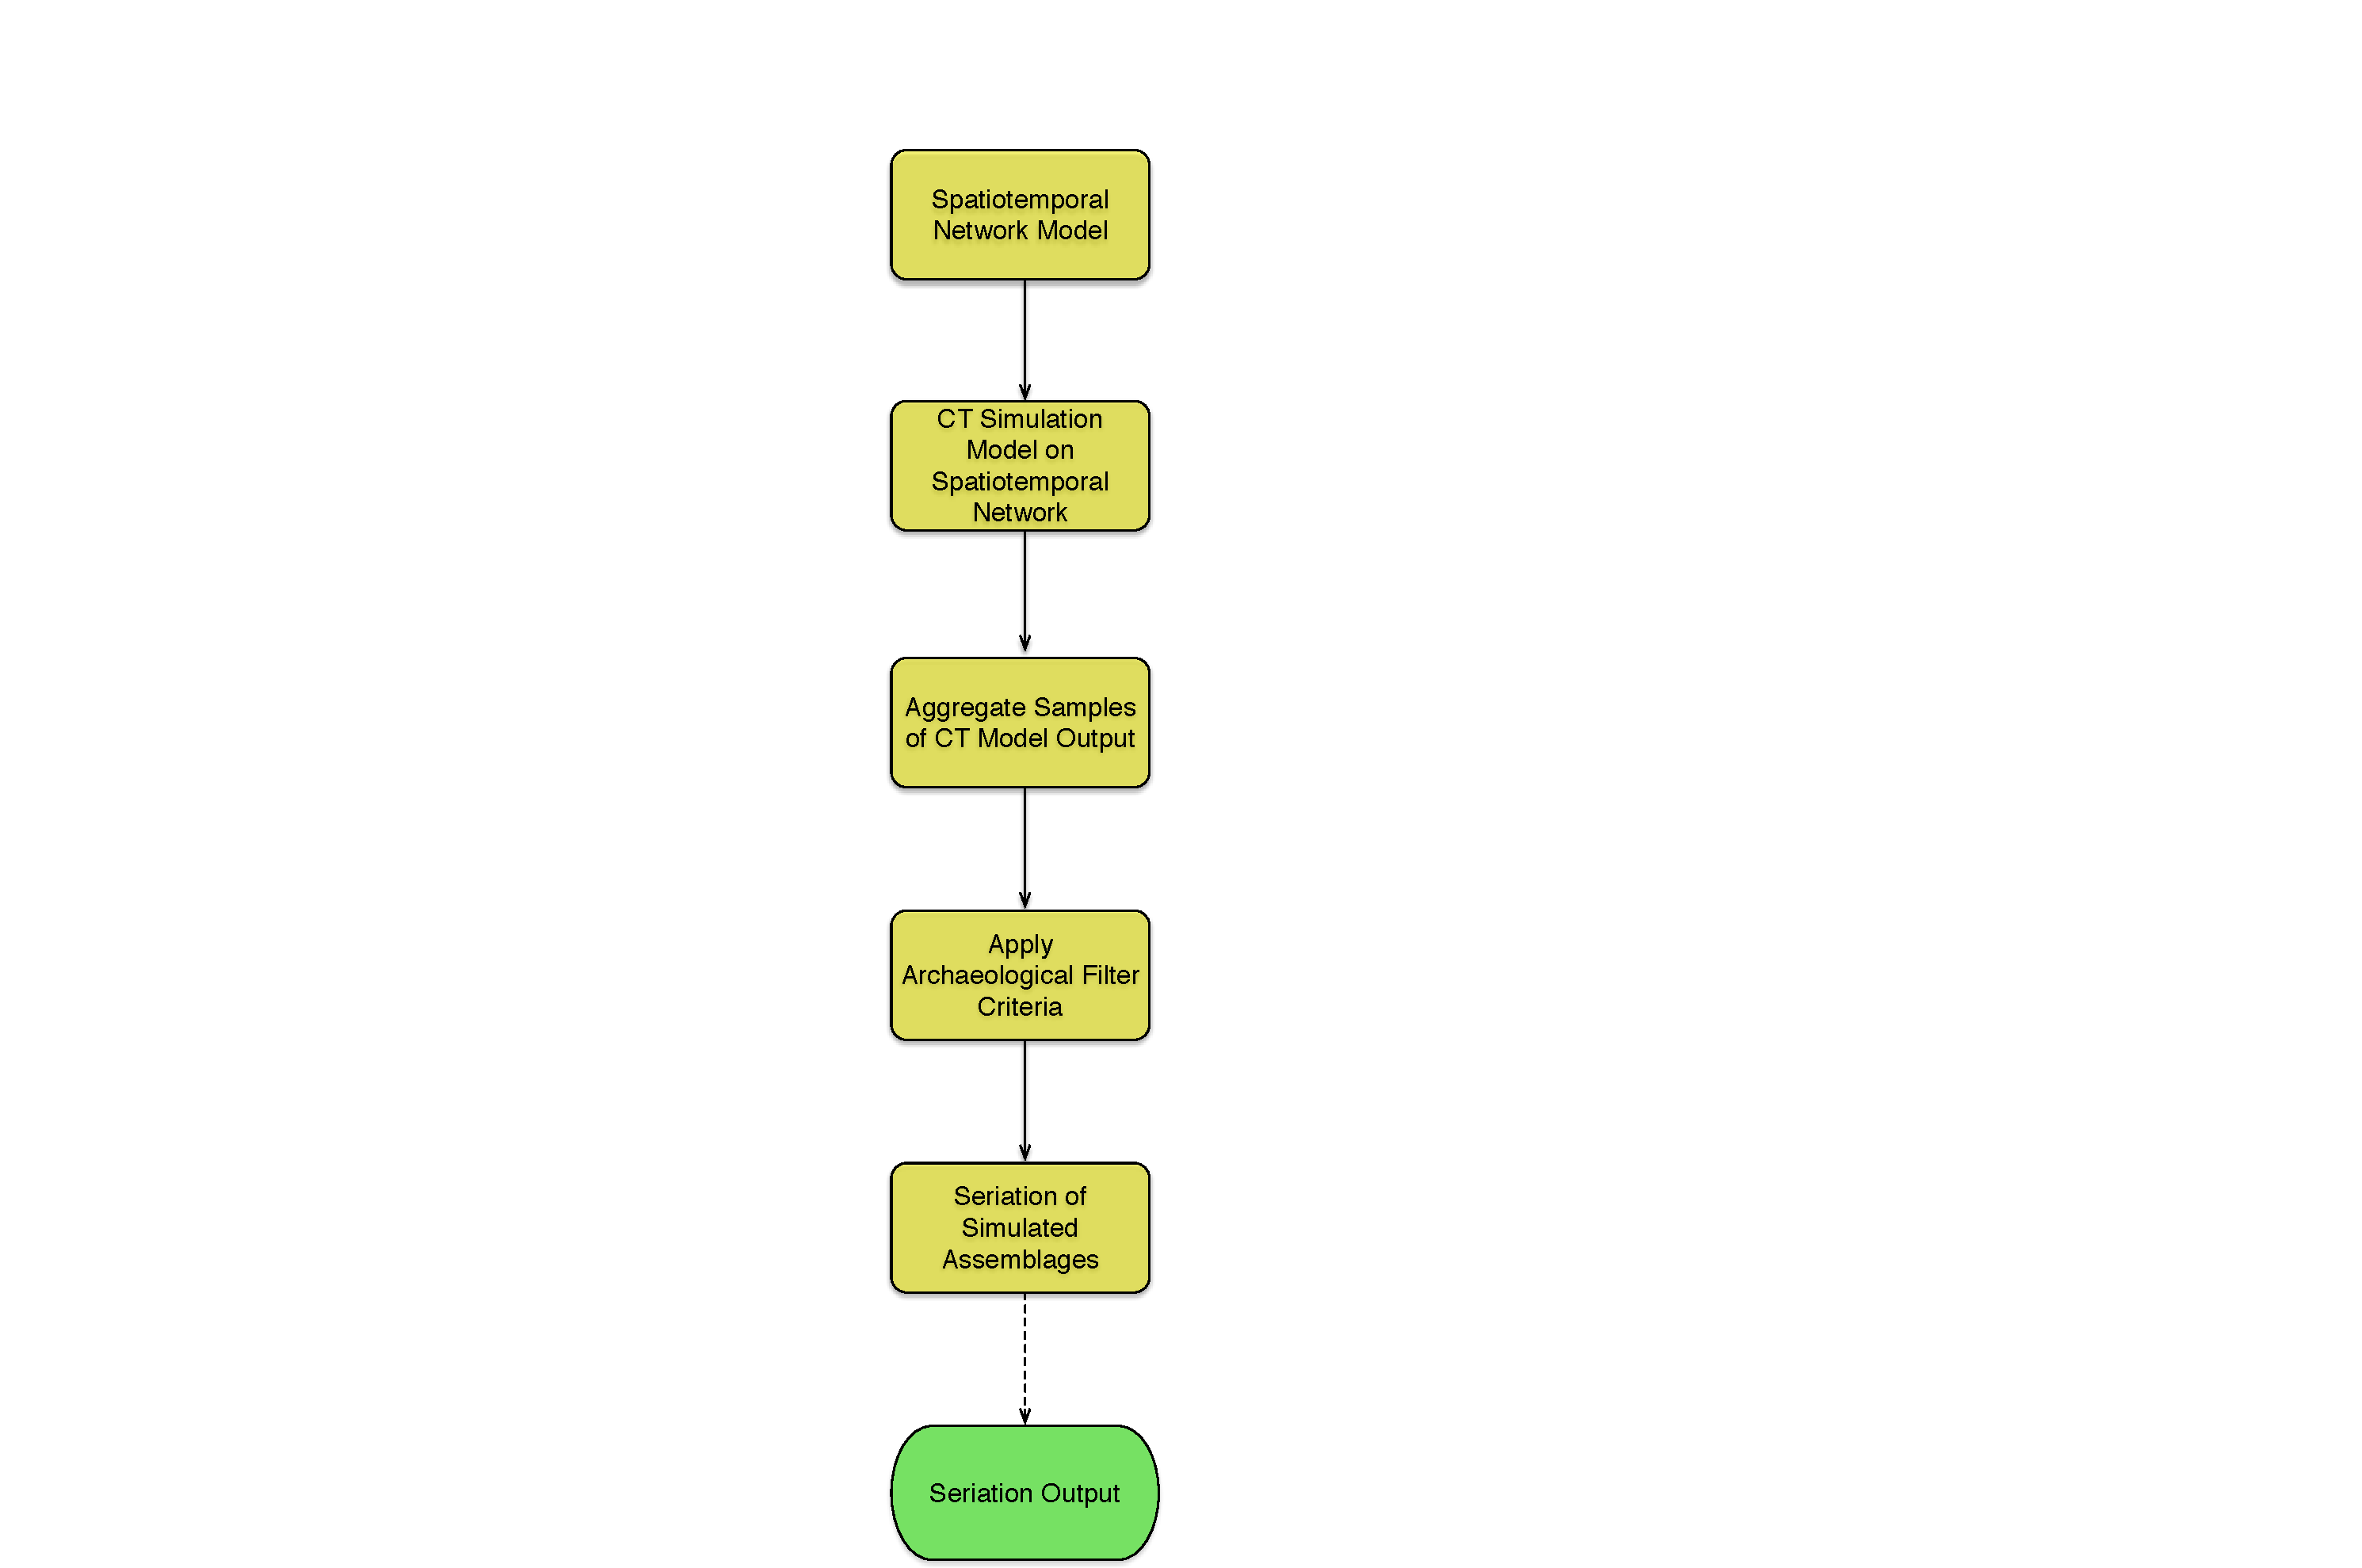
\includegraphics[scale=0.4]{seriationct-high-level-flow.pdf}
\caption{Processing steps in simulating cultural transmission on a regional metapopulation model of lineage splitting, to compare seriation ordering algorithms.}
\label{img:seriationct-flow}
\end{figure}

Following simulation and data recording, the raw data are processed in
ways that mimic the time averaging that occurs in archaeological
deposits, and the sampling that archaeologists do when taking surface
collections from such aggregated deposits. This chain of processing is
depicted in Figure \ref{img:seriationct-flow}. First, recorded cultural
variants are aggregated for each community across the simulated time
that community existed, so that all variant frequencies are time
averaged in the manner described and modeled by Premo
\citeyearpar{Premo2014} and Madsen \citeyearpar{Madsen2012}. Then, from
the time averaged data for each community, an assemblage of 500
simulated artifacts is drawn from the raw data. This has a tendency to
represent common variants well, and capture some but not all rare
variants. From this sampled data, we then take a sample of the available
communities, since seriations are always performed on a sample of
archaeological deposits selected by the archaeologist (whether in
rigorous or ad hoc ways). Finally, we filter the types present in each
group of assemblages, to remove those types which are present only in
one assemblage (as one would do in a manually constructed seriation),
since those types do not contribute to ordering.

The resulting set of assemblage-level type frequencies were then fed
into our IDSS seriation program, asking it to produce both a frequency
seriation using unimodality as the ordering criterion, and a continuity
seriation, using exact distance minimization as the ordering criterion.
We did this for 50 simulation runs with different parameters across the
``lineage splitting'' regional model described above, and compared the
resulting seriation solutions.

\section{Discussion}\label{discussion}

Lorem ipsum dolor sit amet, consectetur adipiscing elit. Vestibulum
viverra est est. Proin eget tellus metus. Aenean ac tortor pharetra
libero ultricies sagittis. Nulla facilisi. Cras tincidunt interdum
tellus, quis consectetur nunc facilisis nec. Sed fermentum erat a ligula
posuere quis semper risus ullamcorper. Morbi vel tincidunt augue. Nam
dolor ipsum, sagittis quis dignissim eu, pulvinar sed magna. In interdum
magna eu orci facilisis congue. Cras a tellus et lorem sagittis viverra.
Donec risus lectus, mollis at dignissim viverra, dapibus a nulla.
Vivamus porttitor scelerisque turpis, eget lobortis orci auctor eget.
Donec ultricies enim ac augue porttitor convallis. Pellentesque nisl
lorem, consequat a facilisis in, ornare sed lorem. In luctus, elit ac
mattis dapibus, lacus elit varius tortor, vel sollicitudin massa nisl id
massa. Ut sit amet nibh a sem egestas sollicitudin. Vestibulum
scelerisque, dui at tincidunt accumsan, ipsum enim feugiat neque, vel
interdum turpis lectus sed nisi. Nullam ultrices sodales sem, et
placerat nunc euismod eu. Duis leo lacus, semper quis eleifend vitae,
viverra ut nisl. Vestibulum ante ipsum primis in faucibus orci luctus et
ultrices posuere cubilia Curae; Proin rutrum eleifend est, id tempor
velit viverra sed.


%% References with bibTeX database:

\bibliographystyle{model2-names}
\bibliography{saa2016-seriation-multiple-approaches}

\end{document}
